%\documentclass[twoside]{nwpu}
%\documentclass[openany]{nwpu}   % openany 去掉章节后的空白页 但是不能去掉目录及titlepage的空白页
\documentclass{nwpu}
\begin{document}

    % �������ı��⼰������Ϣ��
\titleC{NWPU ����\TeX{}ģ��˵��}{v0.01}             % ���ı���     �﷨��  \titleC{}{}
\majorC{Χ��}                                       % רҵ         �﷨��  \majorC{}
\authorC{���ٹ�}                                    % ����         �﷨��  \authorC{}
\supervisorC{����}                                  % ��ʦ         �﷨��  \supervisorC{}
\dateC{1014~��~12~��}                               % ����         �﷨��  \dateC{}
\authorno{10141212}                                 % ѧ��         �﷨��  \authorno{}
\secretlevel{����}                                  % �ܼ�         �﷨��  \secretlevel{}
\classno{A0001}                                     % �����       �﷨��  \classno{}
\titleE{How to Use NWPU Paper Template of \TeX}     % Ӣ�ı���     �﷨��  \titleE{}
\majorE{Go}                                         % רҵ(Ӣ��)   �﷨��  \majorE{}
\authorE{Shindou Hikaru}                            % ����(Ӣ��)   �﷨��  \authorE{}
\supervisorE{Sai}                                   % ��ʦ(Ӣ��)   �﷨��  \supervisorE{}
\dateE{December 1014}                               % ����         �﷨��  \dateE{}

\makecover % ���ɷ���


    \frontmatter
    \pagenumbering{Roman}
    % abstract.tex
% 中英文摘要页
%

% 中文摘要页
\begin{abstract}
    为了使作者更加专注于论文的书写而不是格式的排版, 我们提供了nwpu文类, 对毕业论文进行排版. 该文类根据《西北工业大学博士研究生学位论文编写规则(试用版)》编写, 使用了book文类和一些相关宏包.
    \begin{keyword}
        nwpu,  文类, 模板
    \end{keyword}
\end{abstract}

% 英文摘要页
\begin{abstractE}
    According to {\it The Rule of NWPU Paper}, we write this template with a class file nwpu.cls, which can make the author focusing on the content of the paper.
    \begin{keywordE}
        nwpu, class, template
    \end{keywordE}
\end{abstractE}



    \tableofcontents \addcontentsline{toc}{chapter}{目 \quad 录}

    \mainmatter
    \chapter{简介}
        \section{运行环境要求}
            系统已安装 CTeX~2.9.2,并有相应的宏包。
            当前该文类文件只在安装用 CTeX~2.9.2 的 windows 下测试通过。
        % end of section{系统要求}

        \section{模板结构}
            \subsection{文件说明}
                各文件的简要说明见表\ref{maker}:

                \begin{table}[ht]
                    \centering
                    \caption{模板文件名称及作用}\label{maker}
                    \begin{tabular}{rl}
                        \topline
                        {\bf 文件名称} & {\bf 功能描述} \\
                        \hline
                        nwpu.cls & 文类文件,对论文封面及整体风格进行定义 \\
                        nwpu.bst & 用于 BibTeX 的格式文件 \\
                        Tex模板说明.tex & 该模板文件的主体部分 \\
                        cover.tex & 该模板文件的封面内容的定义和封面的生成 \\
                        abstract.tex & 该模板的摘要部分 \\
                        reference.bib & 该模板的参考文献库 \\
                        \bottomline
                    \end{tabular}
                \end{table}

            % end of subsection{目录结构}
        % end of section{模板结构}
    % end of chapter{简介}

    \chapter{使用说明}
        \section{模板框架介绍}
            下面是模板文件的整体框架部分:
            %\begin{center}
                \vskip 10pt
                \hskip 1cm
                \begin{minipage}[t]{8cm}
                    \zihao{5}\it
                    01 \qquad\textbackslash documentclass[a4paper]\{nwpu\}   \par
                    02 \qquad\textbackslash begin\{document\}                \par
                    03 \qquad\textbackslash include \{cover\}                \par
                    04 \                                               \par
                    05 \qquad\textbackslash frontmatter                      \par
                    06 \qquad\textbackslash include\{abstract\}              \par
                    07 \qquad\textbackslash tableofcontents                  \par
                    08 \                                               \par
                    09 \qquad\textbackslash mainmatter                       \par
                    10 \qquad\textbackslash include\{chapter1\}              \par
                    11 \qquad\% \textbackslash include\{chapter2\}           \par
                    12 \qquad\% \textbackslash include\{chapter3\}           \par
                    13 \                                               \par
                    14 \qquad\textbackslash backmatter                       \par
                    15 \qquad\textbackslash bibliographystyle\{nwpu\}        \par
                    16 \qquad\textbackslash bibliography\{reference\}        \par
                    17 \qquad\textbackslash end\{document\}                  \par
                \end{minipage}
                \par
                \vskip 20pt
            %\end{center}
            下面我们根据以上代码对各部分的功能和书写方法进行说明。第1行加载文类文件nwpu.cls, 和一般文类文件的使用方法相同\footnote{我们建议文件开头写法如下:\framebox{\bf\textbackslash documentclass\{nwpu\}}}。第2行标识着文档的开始(而第17行与之相对, 标识着文档的结束)。第3行引用了外部文件cover.tex, 该文件中我们需要填写论文封面需要的一些信息,包括论文标题,作者,作者专业,指导老师,日期等信息\footnote{请打开cover.tex 查看其需要的字段及各字段的意义}。第6行引用了外部文件abstract.tex, 该文件只包含中英文摘要和其关键字。第10--12行, 引用外部文件chapter1.tex, 这是正文部分, 和 book 文类的 chapter 写作方法相同。第15--16行用于参考文献的引用,该部分需要使用BiBTex\cite{LatexCompanion}。

            \begin{equation} 
                a^2 + b^2 = (a + b)^2 -2ab
            \end{equation}
            \begin{equation}
                F(x) = \int_a^b f(x) dx
            \end{equation}
            \begin{figure}
              \centering
              % Requires \usepackage{graphicx}
              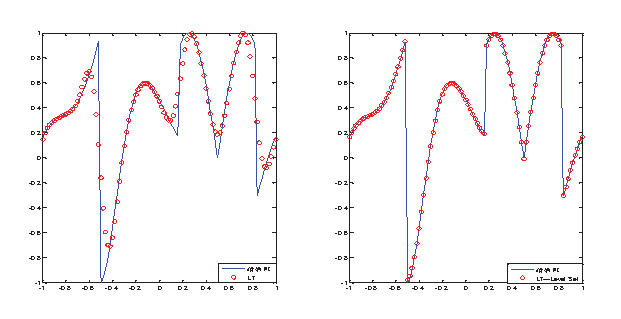
\includegraphics[width=8cm]{11.eps}\\
              \caption{测试小图而已}\label{figOne}
            \end{figure}


        % end of section{文类文件nwpu.cls}
    % end of chapter{使用说明}

    %\chapter{注意事项}
        % end of section{Test cite}
    % end of chapter{注意事项}

    \backmatter

    \bibliographystyle{nwpu}  % nwpu.bst
    \bibliography{reference}  % reference.bib

    \chapter{附 \quad 录}

    \chapter{致 \quad 谢}

    \chapter{攻读博士学位期间发表的学术论文和参加科研情况}
    % 这里如何自动生成?

    \statement  % 知识产权声明

\end{document}

